\documentclass[11pt, oneside]{article}   	% use "amsart" instead of "article" for AMSLaTeX format
%\usepackage{geometry}                		% See geometry.pdf to learn the layout options. There are lots.
%\geometry{letterpaper}                   		% ... or a4paper or a5paper or ... 
%\geometry{landscape}                		% Activate for rotated page geometry
%\usepackage[parfill]{parskip}    		% Activate to begin paragraphs with an empty line rather than an indent

\usepackage{geometry}
 \geometry{
 a4paper,
 total={170mm,257mm},
 left=20mm,
 top=20mm,
 bottom=20mm,
 }

\usepackage{graphicx}				% Use pdf, png, jpg, or eps§ with pdflatex; use eps in DVI mode
								% TeX will automatically convert eps --> pdf in pdflatex		
\usepackage{amssymb}
\usepackage{amsmath}
\usepackage{fancyhdr}
\usepackage[utf8]{inputenc}
\usepackage[english]{babel}
\usepackage{enumerate}
\usepackage{arcs}
\usepackage{cancel}
\usepackage{xfrac}
\usepackage{soul}
\usepackage{tikz}

%SetFonts

%SetFonts

\usepackage[inline]{asymptote}


\newtheorem{theorem}{Theorem}
\pagestyle{fancy}
\fancyhf{}
\rhead{Cindy Hu}
\lhead{\leftmark}


\title{Lecture Notes}
\author{Cindy Hu}
%\date{}							% Activate to display a given date or no date

\begin{document}
\maketitle




\section{Quadratic Equations}
\subsection{Solving Equations By Completing Square}
Given quadratic equation $ax^2+bx+c=0, a \ne 0, a, b, c \in \mathbb{R}$, we can solve it by the technique of \emph{Completing Square}: 
\begin{align*}
& ax^2+bx+c=0\\
\Rightarrow \quad & x^2+\frac{b}{a}x+\frac{c}{a}=0\\
\Rightarrow \quad & (x+\frac{b}{2a})^2-\frac{b^2}{4a^2}+\frac{c}{a}=0\\
%\Rightarrow \quad & (x+\frac{b}{2a})^2=\frac{b^2}{4a^2}-\frac{c}{a}\\
\Rightarrow \quad & (x+\frac{b}{2a})^2=\frac{b^2-4ac}{4a^2}\\
\Rightarrow \quad & x+\frac{b}{2a}=\pm \frac{\sqrt{b^2-4ac}}{2a}\\
\Rightarrow \quad & x=\frac{-b \pm \sqrt{b^2-4ac}}{2a}\\
\end{align*}

This is the formula commonly known for solving quadratic equations. Obviously, the equation has \hl{real solutions only if $b^2-4ac \ge 0$}. Specifically, \hl{when $b^2-4ac = 0$, the equation has two identical roots}. \\


\subsection{Factorisation}


If equation $ax^2+bx+c = 0$ has two roots $\alpha$ and $\beta$, then the equation can be \hl{factorised} as $a(x-\alpha)(\alpha-\beta)=0$. Therefore, if the equation can be easily factorised, we are able to solve it \hl{without using the formula introduced in the previous section}. 

For example, given equation $3x^2 - 8x +4=0$, if we want to factorise $3x^2 - 8x +4$, we firstly factorise the coefficient of the highest term $3x^2$, and factorise the constant term 4. For term $3x^2$, the coefficient is 3. It can be factorised as $1 \times 3$ or $-1\times -3$. For constant term 4, it can be factorised as $1 \times 4$, $-1\times -4$, $2\times 2$, or $-2\times -2$. 


\begin{figure}
\centering 
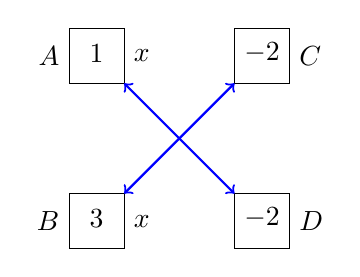
\begin{tikzpicture} [scale=0.7]

\draw (0,0) -- (0,1) -- (1,1) -- (1,0) -- cycle; 
\draw (3,0) -- (3,1) -- (4,1) -- (4,0) -- cycle; 
\draw (0,3) -- (0,4) -- (1,4) -- (1,3) -- cycle; 
\draw (3,3) -- (3,4) -- (4,4) -- (4,3) -- cycle; 

\draw [<->, blue, thick] (1,3)--(3,1);
\draw [<->, blue, thick] (1,1)--(3,3);

\coordinate [label=left:$A$](a) at(0, 3.5);
\coordinate [label=left:$B$](b) at(0, 0.5);
\coordinate [label=right:$C$](c) at(4, 3.5);
\coordinate [label=right:$D$](d) at(4, 0.5);

\coordinate [label=$1$](a1) at(0.5, 3.2);
\coordinate [label=$3$](b1) at(0.5, 0.2);
\coordinate [label=$-2$](c1) at(3.5, 3.2);
\coordinate [label=$-2$](d1) at(3.5, 0.2);

\coordinate [label=right:$x$](a2) at(1, 3.5);
\coordinate [label=right:$x$](b2) at(1, 0.5);

\end{tikzpicture}
\caption{Factorization of $3x^2 - 8x + 4$}
\label{fig:factorization}
\end{figure}


To make it illustrative, we usually use a \hl{square diagram} to fulfill the task.  As illustrated in Figure~\ref{fig:factorization}, we put the factors of 3 into squares $A$ and $B$, and put the factors of 4 into squares $C$ and $D$, we then cross-multiply $AD$ and $BC$ such that $AD + BC$ equals -8, the coefficient of the term $-8x$.  Figure~\ref{fig:factorization} illustrates the correct way to factorize $3x^2 -8x +4$. $AB$ implies that the term $3x^2$ is factorised as $x \times 3x$. $CD$ implies that 4 is factorised as $-2 \times -2$. $AC$ together means that we get $(x-2)$, $BD$ together means that we get $(3x-2)$. Eventually, $3x^2 - 8x +4 = (x-2)(3x-2)$. 

To solve $3x^2 - 8x +4=0$, we then have $x-2=0$ or $3x-2=0$. The two roots are $x=2$ and $x=\frac{2}{3}$. 

Unfortunately, not every quadratic equation can be factorised in such a clean way. But if we do meet an equation which we find can be factorised, solving it by factorisation would save quite a bit of effort. 

\subsection{the Relationship Between Roots and Coefficients}

Given quadratic equation $ax^2+bx+c=0$, if there exits \hl{two roots $\alpha$ and $\beta$}, then the equation can be written in a factorized form as 
\[a(x-\alpha)(x-\beta) = 0.\] 

Expanding the above equation, we have 
\[ax^2-a(\alpha+\beta)+a\alpha\beta=0.\]
Comparing $ax^2-a(\alpha+\beta)+a\alpha\beta=0$ with $ax^2+bx+c=0$, we realise that 
\[b=-a(\alpha+\beta)\quad  \text{ and } \quad c=a\alpha\beta.\] 
We often write the above in a slightly different way 
\[\alpha+\beta=-\frac{b}{a}, \quad  \text{ and } \quad \alpha\beta=\frac{c}{a},\] 
which is also known as \hl{Vieta's Formula}. 

\subsection{Quadratic Function} 
Given quadratic function $f(x)=ax^2+bx+c, a\ne 0, a, b, c \in\mathbb{R}$, it's curve is a parabola in in a two-dimensional space. The value of $a$ determines which direction the parabola opens to. \hl{If $a>0$, the parabola opens upward, if $a<0$, the parabola opens downwards}. 

\subsection{the Vertex Form} 

Given the quadratic equation: 
\begin{align*}
f(x) &=ax^2+bx+c\\
& =a\left(x^2+\frac{b}{a}\right)x+c\\
& =a\left(x+\frac{b}{2a}\right)^2+c-\frac{b^2}{4a}\\
& =a\left(x+\frac{b}{2a}\right)^2+\frac{4ac-b^2}{4a^2}\\
\end{align*}

\subsubsection{What does the vertex form disclose? }
The vertex form discloses the following:
\begin{enumerate}
\item The curve of $f(x)$ is symmetric.

\item The axis of symmetry is $x=-\frac{b}{2a}$. 

\item \hl{The vertex of $f(x)$ is $(-\frac{b}{2a}, \frac{4ac-b^2}{4a})$. When $a>0$, $\frac{4ac-b^2}{4a}$ is the minima of $f
(x)$; when $a<0$, $\frac{4ac-b^2}{4a}$ is the maxima. }

\end{enumerate} 

\subsection{Another Way to Solve Quadratic Equation}
Given quadratic equation  $3x^2-6x-1=0$, solving the equation is equivalent to finding the intersection points of $f(x) =3x^2 -6x -1$ to the $x$-axis. If the intersections are $(x_1, 0)$ and $(x_2, 0)$, we can plot the parabola  of $f(x)$, as illustrated in Figure~\ref{fig:parabola}. The axis of symmetry is $x = -\frac{-6}{2\times 3} = 1$. 

Assuming the distance between $x_1$ and $x_2$ is $2d$, then $x_1 = 1-d$ and $x_2 = 1+d$, apparently. $x_1$ and $x_2$ will be solved once we figure out the value of $d$. 

By \emph{Vieta's Formula}, we have $x_1\cdot x_2 = \frac{-1}{3}$, which implies 
\begin{align*}
&(1-d)(1+d) = -\frac{1}{3}\\
\Rightarrow \quad & 1-d^2 = -\frac{1}{3}\\
\Rightarrow \quad & d^2 = \frac{4}{3}\\
\Rightarrow \quad & d= \sqrt{\frac{4}{3}} = \frac{2}{3}\sqrt{3}
\end{align*}

Finally, we have
\[x_1= 1-\frac{2}{3}\sqrt{3}, \quad x_2 = 1+\frac{2}{3}\sqrt{3}.\]

\begin{figure}
\centering 
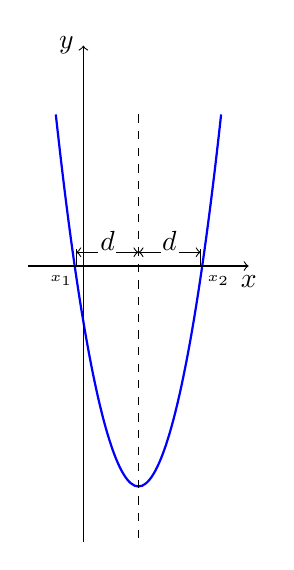
\begin{tikzpicture} [scale=0.7]

\draw [blue, thick] (-0.5,2.75) parabola bend (1,-4) (2.5,2.75);
\draw [->] (-1,0)--(3,0);
\draw [->](0,-5)--(0,4);
\draw [dashed] (1, 2.75) -- (1,-5);
\draw (2.13,0) -- (2.13,0.3);
\draw (-.13,0) -- (-.13,0.3);
\draw [<-](-0.13,0.25) --(0.27,0.25);
\draw [->](0.6,0.25) --(1,0.25);

\draw [<-](1,0.25) --(1.4,0.25);
\draw [->](1.73,0.25) --(2.13,0.25);

\coordinate [label=above:$d$](d1) at (0.44,0.1);
\coordinate [label=above:$d$](d2) at (1.56,0.1);

\coordinate [label=below:{\tiny $x_1$}](x1) at (-0.4,0);
\coordinate [label=below:{\tiny $x_2$}](x2) at (2.45,0);

\coordinate [label=below:$x$](x) at (3,0);
\coordinate [label=left:$y$](y) at (0,4);

\end{tikzpicture}
\caption{Parabola of $3x^2 - 6x -1$}
\label{fig:parabola}
\end{figure}

\newpage
\section{Symmetric Polynomial}
A symmetric polynomial is a polynomial where if you switch any pair of variables, it remains the same. For example, $x^2+y^2+z^2$ is a symmetric polynomial, since switching any pair, say $x$ and $y$, the resulting polynomial $y^2+x^2+z^2$ is the same as the initial polynomial. Symmetric polynomials are closely related to Vieta's formula and Newton's identities. 


\subsection{Elementary Symmetric Polynomial}
\begin{theorem}
Any symmetric polynomial can be presented by elementary symmetric polynomial. 
\end{theorem}

Elementary symmetric polynomials are the building blocks for all symmetric polynomials. There are $n$ different elementary symmetric polynomials for $n$ variables, \{$x_1,x_2,\dots ,x_n$\}, and we define them as \{$e_1, e_2, \dots ,e_n$\}: 
\begin{align*}
e_1 &=\sum_{1\le i\le n} x_i\\
e_2 &=\sum_{1\le i< j\le n} x_i x_j\\
\vdots\\
e_n &=x_1 x_2 \cdots x_n\\
\end{align*}
 
For example, there are two variables $a$ and $b$. Their elementary symmetric polynomials are: 
\begin{align*}
e_1 &=a+b\\
e_2 &=ab\\
\end{align*}

If there are three variables $a$, $b$, and $c$, their elementary symmetric polynomials are: 
\begin{align*}
e_1 &=a+b+c\\
e_2 &=ab+bc+ca\\
e_3 &=abc \\
\end{align*}

Given Symmetric Polynomial $a^2+b^2-3ab$, it can be presented as:
\[a^2+b^2-3ab = a^2+b^2+2ab-5ab=(a+b)^2-5ab\]

Given Symmetric Polynomial $\frac{1}{a^2}+\frac{1}{b^2}$, it can be presented as:
\[\frac{1}{a^2}+\frac{1}{b^2}=\frac{a^2+b^2}{a^2 b^2}=\frac{(a+b)^2-2ab}{(ab)^2}\] 

Given Symmetric Polynomial $\frac{1}{a^2}+\frac{1}{b^2}+\frac{1}{c^2}$, it can be presented as:
\[\frac{1}{a^2}+\frac{1}{b^2}+\frac{1}{c^2}=\frac{a^2b^2+b^2c^2+c^2a^2}{a^2 b^2c^2}=\frac{(ab+bc+ca)^2-2abc(a+b+c)}{(abc)^2}\] 


%\renewcommand{\labelenumii}{(\arabic{enumii})}


%\begin{enumerate}
%\renewcommand{\labelenumi}{1.\arabic{enumi}}

%\item \label{rule:add} \emph{Addition Principle}. If there are $a$ varieties of soup and $b$ varieties of salad, then there are $a+b$ possible ways to order a meal of soup \emph{or} salad (but not both soup and salad). 

%\end{enumerate}




\end{document} 